
\documentclass{beamer}
\setbeamercolor{frametitle}{fg=white}
\setbeamercolor{title}{fg=white}
\setbeamercolor{author}{fg=white}
\setbeamercolor{date}{fg=white}
\setbeamercolor{normal text}{fg=white}

\useoutertheme{infolines} 
\usepackage{graphicx}
\setbeamertemplate{background}{
\includegraphics[width=\paperwidth,height=\paperheight]{./images/background.png}}

% UTF-8
\usepackage[utf8]{inputenc}

\title{Predstavitev: SlAIdi}
\author{Maša, Tian, Nik}
\institute{Univerza}
\date{\today}

\begin{document}

\begin{frame}
\titlepage
\end{frame}

% Slide 1
\begin{frame}
\frametitle{Kdo smo?}
\begin{itemize}
    \item Avtomatsko ustvarja prosojnice za predstavitve.
    \item Generira tudi skript, po katerem naj bi govorili.
\end{itemize}
\centering

\includegraphics[width=0.5\textwidth]{./images/team.png}
\end{frame}

% Slide 2
\begin{frame}
\frametitle{Kako deluje?}
\begin{itemize}
    \item Povzame vhodni tekst preko API klicev.
    \item Sprejema pozive, skripte ali cele seminarske naloge.
    \item Generira PDF prosojnice, Latex kodo in TXT skript.
\end{itemize}
\centering
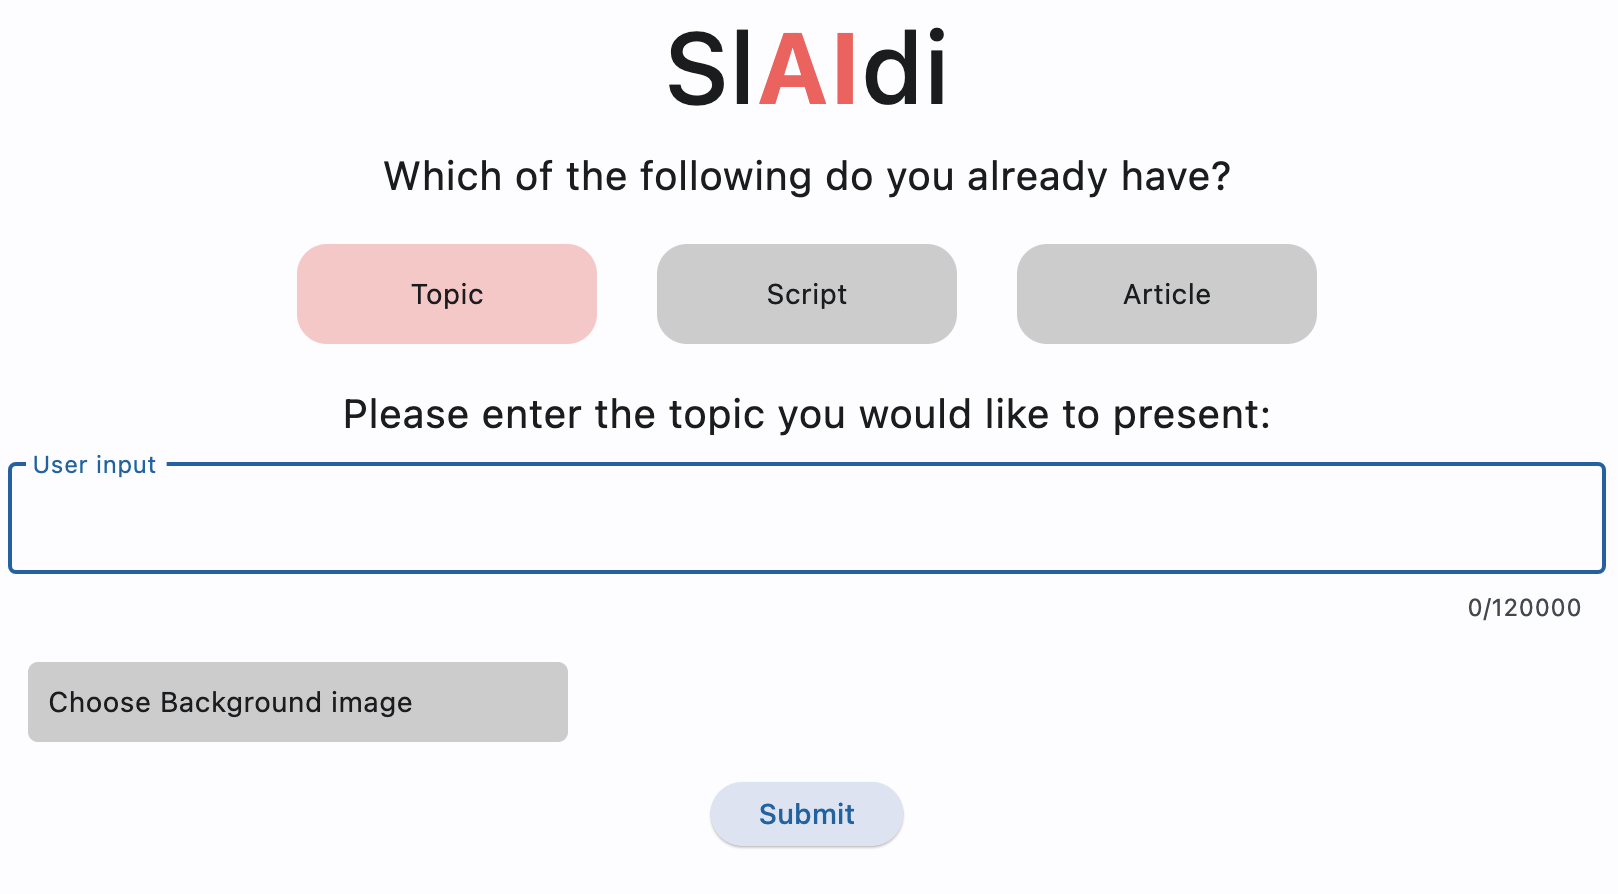
\includegraphics[width=0.5\textwidth]{./images/workflow.png}
\end{frame}

% Slide 3
\begin{frame}
\frametitle{Zakaj ta program?}
\begin{itemize}
    \item Pospeši postopek predstavljanja.
    \item Ni potrebe po pozornosti do malenkosti in ponavljanju.
    \item Uporaben v šoli in podjetjih.
\end{itemize}
\centering
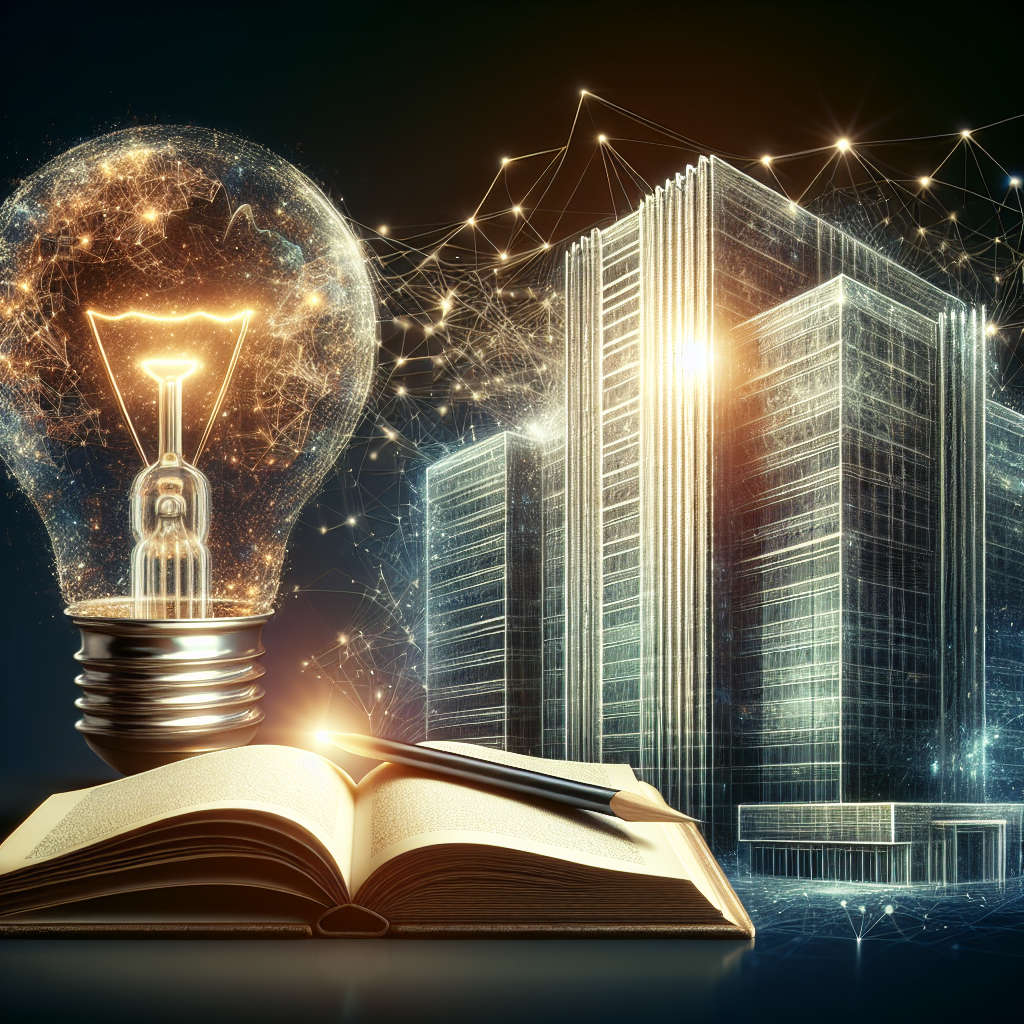
\includegraphics[width=0.5\textwidth]{./images/reasons.png}
\end{frame}

% Slide 4
\begin{frame}
\frametitle{Prilagodljivost}
\begin{itemize}
    \item Omogoča začetno generiranje in naknadne popravke.
    \item Uporabnik lahko spremeni slike in besedilo.
\end{itemize}
\centering

\includegraphics[width=0.5\textwidth]{./images/customize.png}
\end{frame}

% Slide 5
\begin{frame}
\frametitle{Zaupnost in veljavnost}
\begin{itemize}
    \item Celotna predstavitev je narejena s pomojo našega programa.
    \item Ni bilo uporabljeno nobeno drugo orodje.
\end{itemize}
\centering

\includegraphics[width=0.5\textwidth]{./images/trust.png}
\end{frame}

% Slide 6
\begin{frame}
\frametitle{Izbolj�ave}
\begin{itemize}
    \item Trenutno deluje z "image generatorji" za slike.
    \item Za matematične modele in grafe ni popoln.
    \item Možnost dodajanja drugih knjižnic za boljže rezultate.
\end{itemize}
\centering
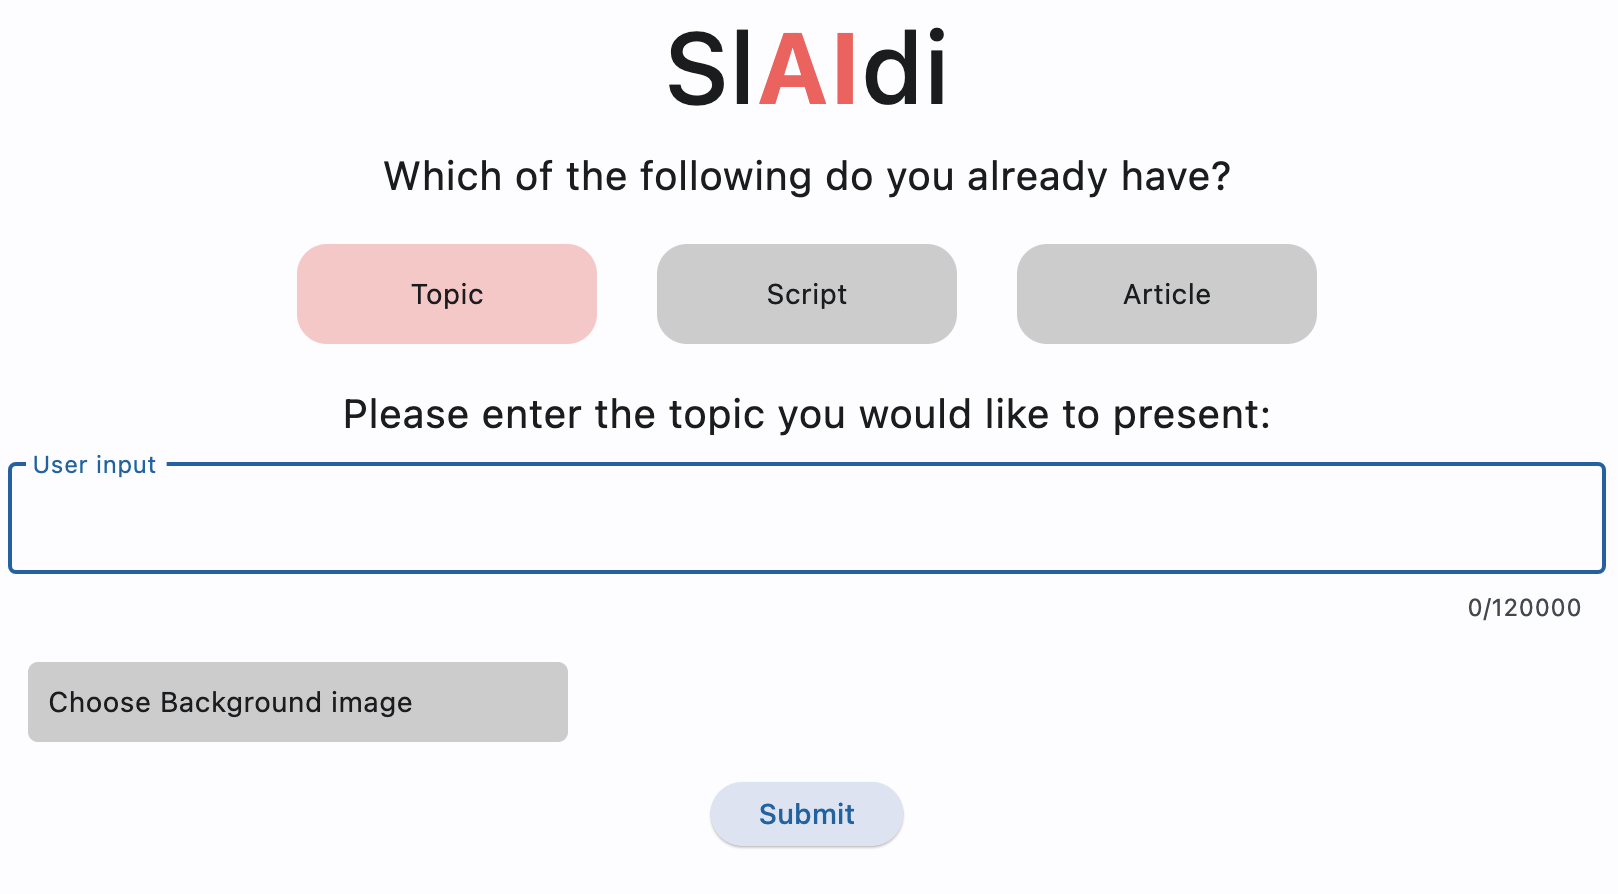
\includegraphics[width=0.5\textwidth]{./images/improvements.png}
\end{frame}

% Closing slides
\begin{frame}
\frametitle{Sklepne misli}
\begin{itemize}
    \item SlAIdi avtomatizira ustvarjanje predstavitev.
    \item Prilagaja in izboljšuje na podlagi uporabnikovih potreb.
    \item Obeta nadaljnje izboljšave in nadgradnje.
\end{itemize}
\centering

\includegraphics[width=0.5\textwidth]{./images/conclusion.png}
\end{frame}

\begin{frame}
\frametitle{Vprašanja?}
\centering

\includegraphics[width=0.5\textwidth]{./images/questions.png}
\end{frame}

\begin{frame}
\frametitle{Hvala za vašo pozornost!}
\centering

\includegraphics[width=0.5\textwidth]{./images/thankyou.png}
\end{frame}

\end{document}
